% !TEX TS-program = pdflatex
% !TEX encoding = UTF-8 Unicode

% This is a simple template for a LaTeX document using the "article" class.
% See "book", "report", "letter" for other types of document.

\documentclass[11pt]{article} % use larger type; default would be 10pt

\usepackage[utf8]{inputenc} % set input encoding (not needed with XeLaTeX)

%%% Examples of Article customizations
% These packages are optional, depending whether you want the features they provide.
% See the LaTeX Companion or other references for full information.

%%% PAGE DIMENSIONS
\usepackage{geometry} % to change the page dimensions
\geometry{a4paper} % or letterpaper (US) or a5paper or....
% \geometry{margin=2in} % for example, change the margins to 2 inches all round
% \geometry{landscape} % set up the page for landscape
%   read geometry.pdf for detailed page layout information

\usepackage{graphicx} % support the \includegraphics command and options

\usepackage{listings}


% \usepackage[parfill]{parskip} % Activate to begin paragraphs with an empty line rather than an indent

%%% PACKAGES
\usepackage{booktabs} % for much better looking tables
\usepackage{array} % for better arrays (eg matrices) in maths
%\usepackage{paralist} % very flexible & customisable lists (eg. enumerate/itemize, etc.)
\usepackage{verbatim} % adds environment for commenting out blocks of text & for better verbatim
\usepackage{subfig} % make it possible to include more than one captioned figure/table in a single float
% These packages are all incorporated in the memoir class to one degree or another...

%%% HEADERS & FOOTERS
\usepackage{fancyhdr} % This should be set AFTER setting up the page geometry
\pagestyle{fancy} % options: empty , plain , fancy
\renewcommand{\headrulewidth}{0pt} % customise the layout...
\lhead{}\chead{}\rhead{}
\lfoot{}\cfoot{\thepage}\rfoot{}

%%% SECTION TITLE APPEARANCE
\usepackage{sectsty}
\allsectionsfont{\sffamily\mdseries\upshape} % (See the fntguide.pdf for font help)
% (This matches ConTeXt defaults)

%\usepackage[colorlinks=true]{hyperref}
\usepackage{hyperref}
\hypersetup{
    colorlinks,
    citecolor=black,
    filecolor=black,
    linkcolor=black,
    urlcolor=black
}

%%% ToC (table of contents) APPEARANCE
\usepackage[nottoc,notlof,notlot]{tocbibind} % Put the bibliography in the ToC
\usepackage[titles,subfigure]{tocloft} % Alter the style of the Table of Contents
\renewcommand{\cftsecfont}{\rmfamily\mdseries\upshape}
\renewcommand{\cftsecpagefont}{\rmfamily\mdseries\upshape} % No bold!

%%% END Article customizations

\usepackage[spanish]{babel}
\usepackage{listings} 
%%% The "real" document content comes below...


\title{\fontsize{30}{0} \bf Lenguaje Ruby}
\author{\\Autores: \\  \\-Cristina Barreno \\ -Sixto Castro \\ -Jordy Vasquez\\ \\}
\thispagestyle{empty}
\begin{document}

\newpage

 
\includegraphics[width=3cm]{./imagenes/Espol.png}{ \fontsize{18}{0} \bf ESCUELA SUPERIOR \\}
\begin{center}
{\fontsize{18}{0} \bf POLITÉCNICA DEL LITORAL\\}
\vspace{2cm}
{\LARGE{ Tema: Investigación de Lenguajes }}\\
\vspace{2cm}
{\LARGE{ Materia: Lenguajes de Programación }}\\
\vspace{2cm}
{\LARGE{  Nombre del grupo en Sidweb: Lenguaje Ruby}}\\ 
\vspace{2cm}
{\LARGE{ Paralelo: 1}}\\
\vspace{2cm}
{\LARGE{Fecha de entrega: \\  Miércoles, 23 de Octubre del 2013}}
\thispagestyle{empty}
\end{center}


\maketitle

\newpage
\tableofcontents % No hace falta un TOC en un artículo corto
\thispagestyle{empty}
\addtocontents{toc}{\protect\thispagestyle{empty}}

\newpage
\begin{center}
 {\fontsize{16}{0} \bf Lenguaje Ruby}
\end{center}

\begin{figure}[h]
\centering
 
\includegraphics[width=2cm]{./imagenes/ruby.jpg}
\caption{Logo de Ruby }\label{Fig:Ruby}
\end{figure}


\section{\fontsize{14}{0} \bf Introducción}

 Ruby  Lenguaje creado por Yukihiro Matsumoto,  combina lo mejor de la orientación a objetos (smalltalk) y la facilidad del scripting (perl) generando un lenguaje dinámico, muy expresivo, potente, fácil de aprender y que permite crear aplicaciones empresariales robustas, estables y seguras ademas de ser  multiplataforma , es decir puede correr en gran cantidad de arquitecturas , hasta en telefonos celulares, y su implementacion es bajo licencia de software libre .


\section{\fontsize{14}{0} \bf Características}

\begin{itemize}

      \item  Ruby es un lenguaje multiplataforma (altamente portable).
      \item  Es fácil de escribir. 
      \item  Es un lenguaje interpretado.
      \item  Es un lenguaje orientado a objetos. Al igual que Java, cada tipo de dato es un objeto.
      \item  Es una mezcla de varios lenguajes tales como Perl, Python, Smalltalk y otros, que definen a Ruby como un lenguaje que integra la programación funcional e imperativa.
      \item  Posee expresiones similares(nivel de lenguaje) a las de Perl
      \item  En Ruby, los métodos se pueden o no ser parte de una clase. Puede ser declarado en cualquier parte del archivo.
      \item  Es capaz de manejar excepciones.
      \item  Se puede manejar hilos (multihilos) sin depender del sistema operativo.

\end{itemize}

\section{\fontsize{14}{0} \bf Historia}
Yukihiro Matsumoto crea  Ruby  en Japon en el año 1993, mientras trabajaba en lenguajes como Perl y PHP, pero se ve tentado en vez de crear un Perl mejorado,  su propio lenguaje combinando asi: \begin{bf}
Perl, Smaltalk, Eiffel y Lisp.
\end{bf} Su nombre proviene como referencia al lenguaje Perl(perla) el cual originalmente deseaba mejorar.\\ \\Se lanza al publico en el año 1995, trayendo asi desarrolladores de todo el mundo, que ven a a Ruby como un lenguaje de exploracion. Tiene un crecimiento lento pero seguro hasta que David Heinemeier Hansson crea el framework Rails , el cual impulsa su crecimiento llevandolo a ser dominado como el
\begin{bf}
" Lenguaje de Progra~maccion del 2006" 
\end{bf} e instalandolo entre los 10 mas populares actualmente.\\ \\


\section{\fontsize{14}{0} \bf Tutorial de Instalación}

Como bien sabemos ruby es un lenguaje multiplataforma por lo que aprenderemos a instalrlo en los diferentes sistemas operativos, asi mismo en todos los casos instalaremos la versión de Ruby {\bf 1.9.3} la cual es la version más estable actualmente, ademas te ofrece una extensa lista de paquetes o gemas compatibles y actualizadas.
\newpage

\begin{itemize}
\item{\bf Ruby en Windows\\ \\}

Para instalar el interprete de Ruby en Windows los podemos hacer desde su página oficil visitando  \url{http://rubyinstaller.org/downloads/}  donde descargaremos el $Ruby Installer$ versión $Ruby 1.9.3-p448$ para una arquitectura de 32 bits, si la arquitectura es de 64 bists puedes descargar la versión $Ruby 2.0.0-p247 (x64)$.\\ \\

{Después que descarguemos el instalador lo ejecutamos como administrador y empezamos la instalación.Aceptamos el contrato de licensia.Vea $Figura 2$.\\ \\
\begin{figure}[h]
\centering
 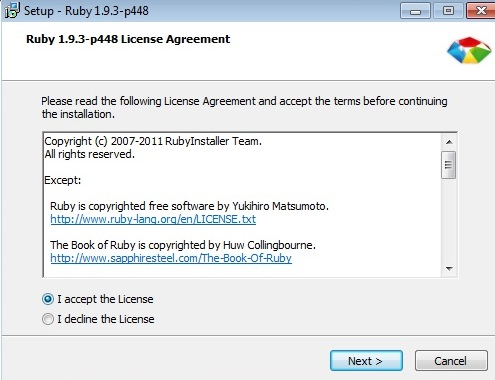
\includegraphics[width=12cm]{./imagenes/PasoInst1.jpg}
\caption{Paso de instalación 1}\label{Fig:Paso1}
\end{figure}}

\newpage
{Agregamos lo necesario para la instalación como se observa en la $ Figura 3$.\\ \\

\begin{figure}[h]
\centering
 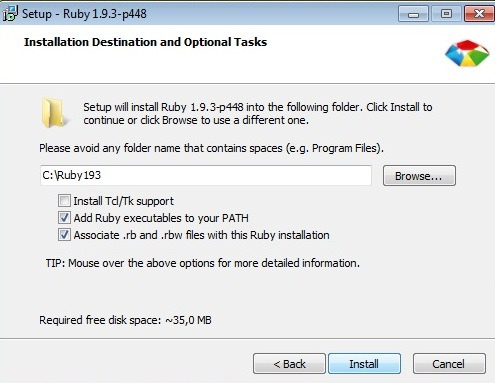
\includegraphics[width=14cm]{./imagenes/PasoInst2.jpg}
\caption{Paso de instalación 2}\label{Fig:Paso2}
\end{figure}}

\newpage
{Terminamos la instalación. Vea  $Figura 4$.\\

\begin{figure}[h]
\centering
 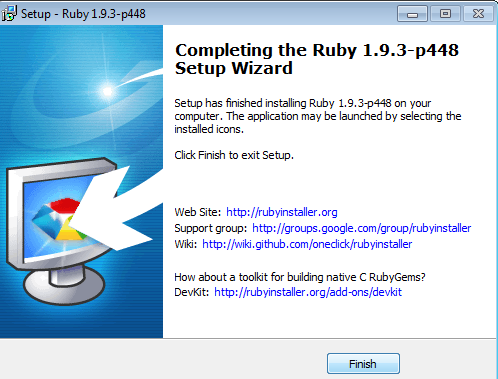
\includegraphics[width=14cm]{./imagenes/PasoInst3.jpg}
\caption{Paso de instalación 3}\label{Fig:Paso3}
\end{figure}}

Abrimos  $Interactive Ruby$ y comenzamos a trabajar con Ruby desde consola. Vea $ Figura 5$.
\begin{figure}[h]
\centering
 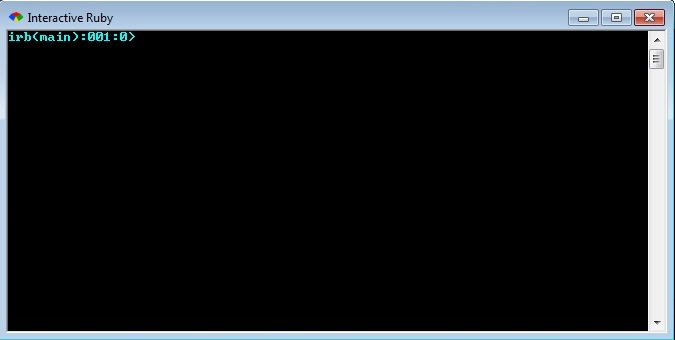
\includegraphics[width=16cm]{./imagenes/PasoInst4.jpg}
\caption{Paso de instalación 4}\label{Fig:Paso4}
\end{figure}

\item{\bf Ruby en Linux}
Dependiendo de la distribución que utilices, hay varias maneras de instalar Ruby. En este caso instalaremos la versión Ruby 1.9.3-p125, para esto necesitaremos abrir una terminal, bajaremos el codigo fuente y lo compilaremos.
En la siguiente página web encontraremos un script con los pasos realizados: \url {http://paste.desdelinux.net/4393}.

\end{itemize}


\section{\fontsize{14}{0} \bf Hola Mundo y otros Programas Introductorios}

A continuación revisaremos algunos programas básicos en ruby para esto solo necesitamos tener instalado en nuestro computador el interprete de ruby, abramos el terminal $ Interactive Ruby$  y empecemos a  programar. Aunque  solo trabajaremos desde consola  recordemos que esta es una herramienta poderosa con la cual daremos nuestros primeros pasos en el mundo de ruby.\\ \\


 {\fontsize{14}{0} \bf Ejemplo 1: Hola Mundo\\}

Para hacer que nuestro programa escriba $"Hola Mundo"$ usaremos el comando $puts Hola Mundo"$,
 siendo  $"puts"$ el comando básico para escribir algo en ruby. \\

          % Set your language (you can change the language for each code-block optionally)

\begin{lstlisting}[frame=single]  % Start your code-block
using System;
     puts  "Hola Mundo"
\end{lstlisting}
\begin{center}
Programa Hola Mundo
\end{center}


 {\fontsize{14}{0} \bf Ejemplo 2: Trabajando con arreglos y Strings \\ }
\begin{itemize}

      \item {\bf Crear un array}\\\\
\begin{lstlisting}[frame=single]  % Start your code-block
using System;
       @names = Array.new
\end{lstlisting}
\begin{center}   
Crea un Array vacío.
\end{center}

      \item {\bf Método [ ]} \\\\
\begin{lstlisting}[frame=single]  % Start your code-block
using System;
     @names = ["Juan", "Luis", "Roberto"]
\end{lstlisting}
\begin{center}
Crea el Array y lo inicializa con strings.
\end{center}
\bf Salida\\\\
    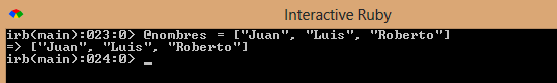
\includegraphics[width=0.9\textwidth]{./imagenes/InicializarArray}\\\\

\newpage

      \item {\bf Método: +}\\\\
\begin{lstlisting}[frame=single]  % Start your code-block
using System;
       @clientes = ["Juan", "Luis", "Roberto"]
       @clientes2 = ["Pierre", "Joe", "Rachel"]
       @clientes + @clientes2
\end{lstlisting}
\begin{center}   
Metodo para unir un array al final de otro.
\end{center}
\bf Salida\\\\
    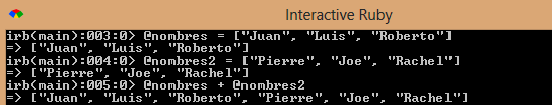
\includegraphics[width=0.9\textwidth]{./imagenes/Metodo+}\\\\
        

     \item {\bf Ordenar un arreglo}\\\\
\begin{lstlisting}[frame=single]  % Start your code-block
using System;
     notasdeberes = [2,4,3,6,8,9,5,1]
     notasdeberes.sort
\end{lstlisting}
\begin{center}
Ordena un Array de menor a mayor.
\end{center}
\bf Salida\\\\
    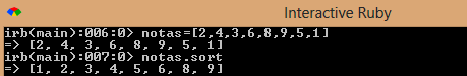
\includegraphics[width=0.9\textwidth]{./imagenes/OrdenarArreglo}\\


\newpage

    \item  {\bf Obtener el tamaño de un arreglo}\\\\
\begin{lstlisting}[frame=single]  % Start your code-block
using System;
     notasdeberes.size()
\end{lstlisting}
\bf Salida\\\\
        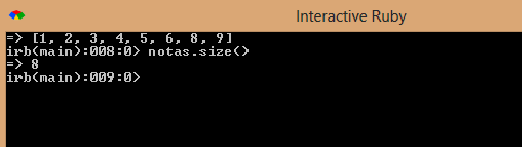
\includegraphics[width=0.9\textwidth]{./imagenes/SizeArreglo}\\\\


     \item  {\bf Recorrer un arreglo: each}\\\\
\begin{lstlisting}[frame=single]  % Start your code-block
equipos = ["Barcelona","Milan","PSG","Monaco"]
equipos.each do |equipo|
  puts equipo
end
\end{lstlisting}
\bf Salida\\\\
        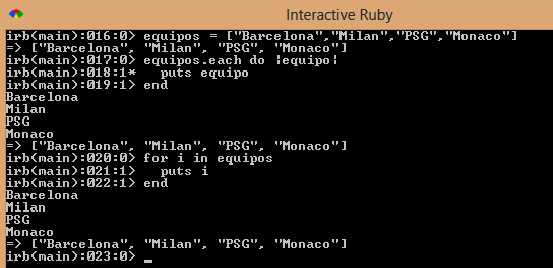
\includegraphics[width=0.9\textwidth]{./imagenes/RecorrerArregloEach}\\\\
     El método 'each' lo que va hacer es recorrer cada elemento del arreglo equipos. En cada iteración, cada elemento del array se guarda en la variable equipo y se va imprimir cada elemento(cadena) del arreglo equipos ya que se encuentra la función puts que se encarga de imprimir cada cadena.\\

	

     \item {\bf Recorrer el arreglo: for in}\\\\
\begin{lstlisting}[frame=single]  % Start your code-block
using System;
for i in equipos
  puts i
end
\end{lstlisting}
\bf Salida\\\\
	    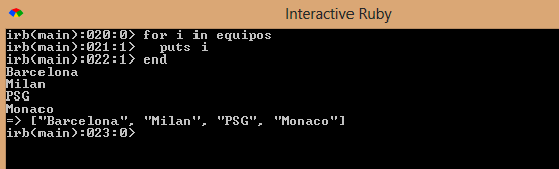
\includegraphics[width=0.9\textwidth]{./imagenes/RecorridoForin}\\\\
     Este caso es parecido al ejercicio anterior, sino que ahora se utiliza un ciclo 'for' para recorrer el arreglo. En cada iteración, la variable 'i' toma el valor actual del array equipos, y luego va imprimir dicho elmento ya que se hace un put en cada iteración.\\
\newpage

    \item {\bf Igualdad entre arreglos}\\\\
\begin{lstlisting}[frame=single]  % Start your code-block
using System;
alumnos1=["Jorge","Luis","Jordy"]
alumnos2=["Orlando","Gabriel","Steven"]
alumnos1=alumnos2
\end{lstlisting}
\bf Salida\\\\
	    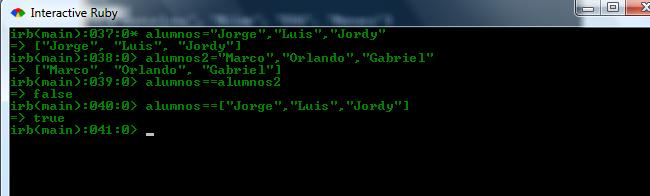
\includegraphics[width=0.9\textwidth]{./imagenes/igualdad_entre_arreglos}\\\\
Devuelve false si no son iguales y true si lo son.\\\\

 {\fontsize{14}{0} \bf Ejemplo 3: Objetos y métodos\\}
  \item {\bf Ejemplo de crear un objeto y un método}\\\\
\begin{lstlisting}[frame=single]  % Start your code-block
using System;
 class Rango
def initialize(caso=0)
@caso=caso
end
def  ver
case @caso
when 1, 2..5
print"el numero esta dentro del rango 1 a 5"
when 6.. 10
print"el numero esta dentro del rango 6 a 10"
else
print"el numero esta fuera del rango"
end
end
end
\end{lstlisting}

	    
Las palabras claves son class para darle el nombre a nuestro objeto,  def  initialize  para inicializarlo , y def ...(y el nombre del metodo) para crear un metodo para el objeto\\\\

  	   \subitem{\bf Utilizando el objeto y su método}\\
\begin{lstlisting}[frame=single]  % Start your code-block
using System;
numero=Rango.new(5)
numero.ver

\end{lstlisting}
\bf Salida\\\\
	    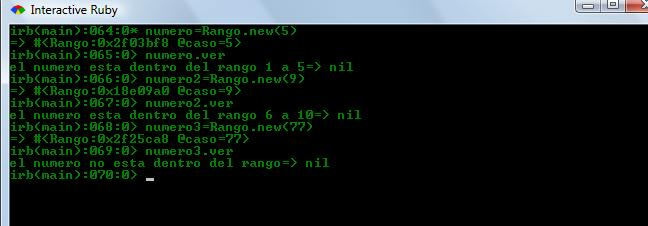
\includegraphics[width=0.9\textwidth]{./imagenes/uso_objecto}\\\\

\bf Salida\\\\
Hacemos una instancia del objeto poniendo el [nombre del objeto].new, e inicializandolo ya sea con vacío o con un valor, y para utilizar el metodo de la misma forma [nombre del objeto].[nombe del método] como muestra Numero2.ver.\\


\end{itemize}

\newpage
\section{\fontsize{14}{0} \bf Referencias}
\begin{itemize}
          \item [1.] https://www.ruby-lang.org/es/about/ \\
          \item [2.] http://es.wikibooks.org/wiki/Programación\_en\_Ruby/Historia\\
	\item[3.]  http://www.maestrosdelweb.com/editorial/la-clase-array-en-ruby/\\
	\item[4.] https://www.ruby-lang.org/es/documentation/quickstart/2/\\
	\item[5.] http://eudev2.uta.cl/rid=1GR0DSG4D-1Y1NH87-4RQ/ruby.pdf\\
	\item[6.] http://www.ecured.cu/index.php/Lenguaje\_de\_Programación\_Ruby\\
	\item[7.]  http://es.wikipedia.org/wiki/Ruby\#Caracter.C3.ADsticas \\
	\item[8.]  http://es.wikibooks.org/wiki/Programación\_en\_Ruby\#Caracter.C3.ADsticas\\
\_Especiales\_del\_Lenguaje \\
	 \item[9.] http://www.ecured.cu/index.php/Lenguaje\_de\_Programación\_Ruby\#Caracter.C3.ADsticas\\
\_generales\_del\_lenguaje \\
	\item[10.] https://www.ruby-lang.org/es/downloads/

\end{itemize}









\end{document}
